\subsection{Who is our target user?}
Our project's (\textit{Magpie's}) primary target is Urban Planners. Urban
Planners are professionals responsible for the development of cities and towns,
focusing on the efficient use of land, infrastructure planning, and the creation
of sustainable and resilient communities. Our secondary target is any casual
user who is interested in amenities planning, and this includes but is not
limited to the following: Sustainability Advocates, Commuters, GIS
professionals, journalists, political advisors, and parking companies.\\

Two main user personas were developed for the context of Magpie's development. \\
These personas serve to guide the feature implementation of Magpie as well as the user evaluation.\\
%michael user persona
\begin{figure}[h!]
    \centering
    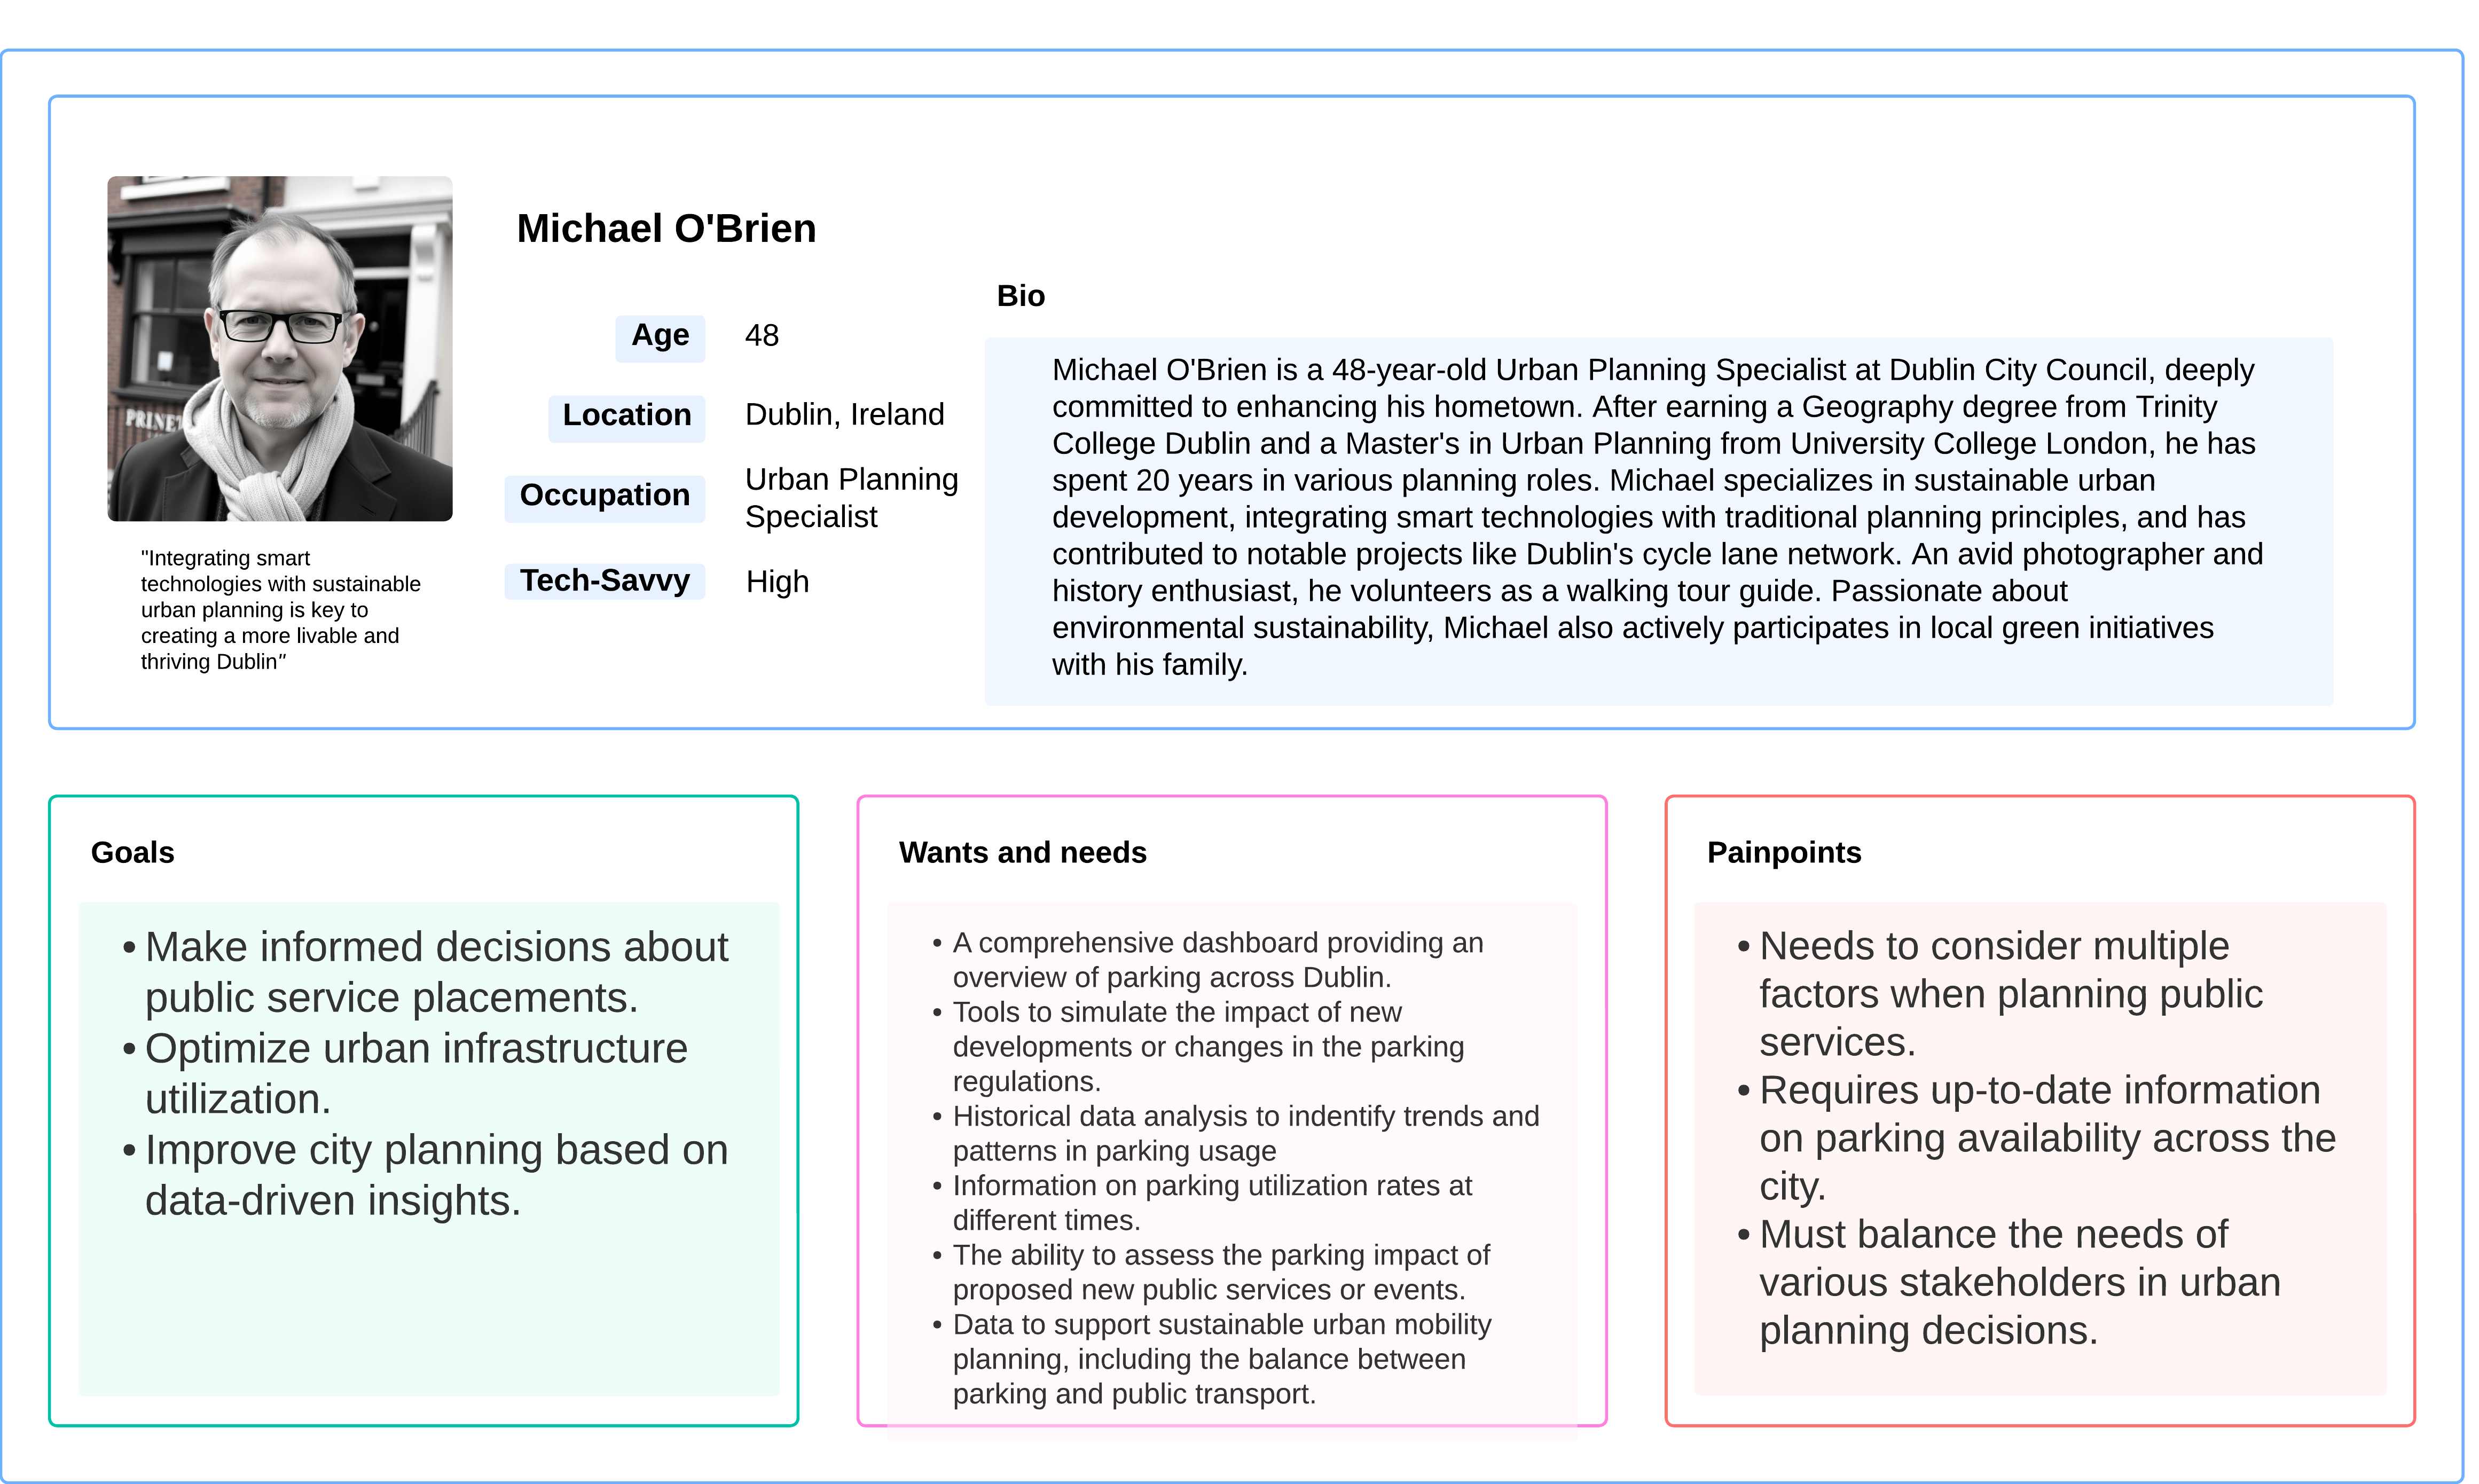
\includegraphics[width=0.8\textwidth]{images/michael-obrien-userpersona.png}
    \caption{User persona - Michael O'Brien}
\end{figure}
Michael O'Brien is a 48-year-old Urban Planning Specialist at Dublin City Council, deeply committed to enhancing his hometown of Lusk. He specializes in sustainable urban development, integrating smart technologies with traditional planning principles, and has contributed to notable projects like Dublin's cycle lane network. He represents our primary target user.\\
Michael is currently working on the expansion of Dublin's cycle lane network southbound. He is facing some challenges because the maps provided by Dublin city council are static and don't show crucial information such as public facilities and amenities. The datasets he's been accessing seem out of date and not comprehensive at all.\\
Michael needs a tool that allows him to interact with a map that contains key data on public facilities and amenities, as well as options to extract that information for analysis and planning.\\

%sarah user persona
\begin{figure}[h!]
    \centering
    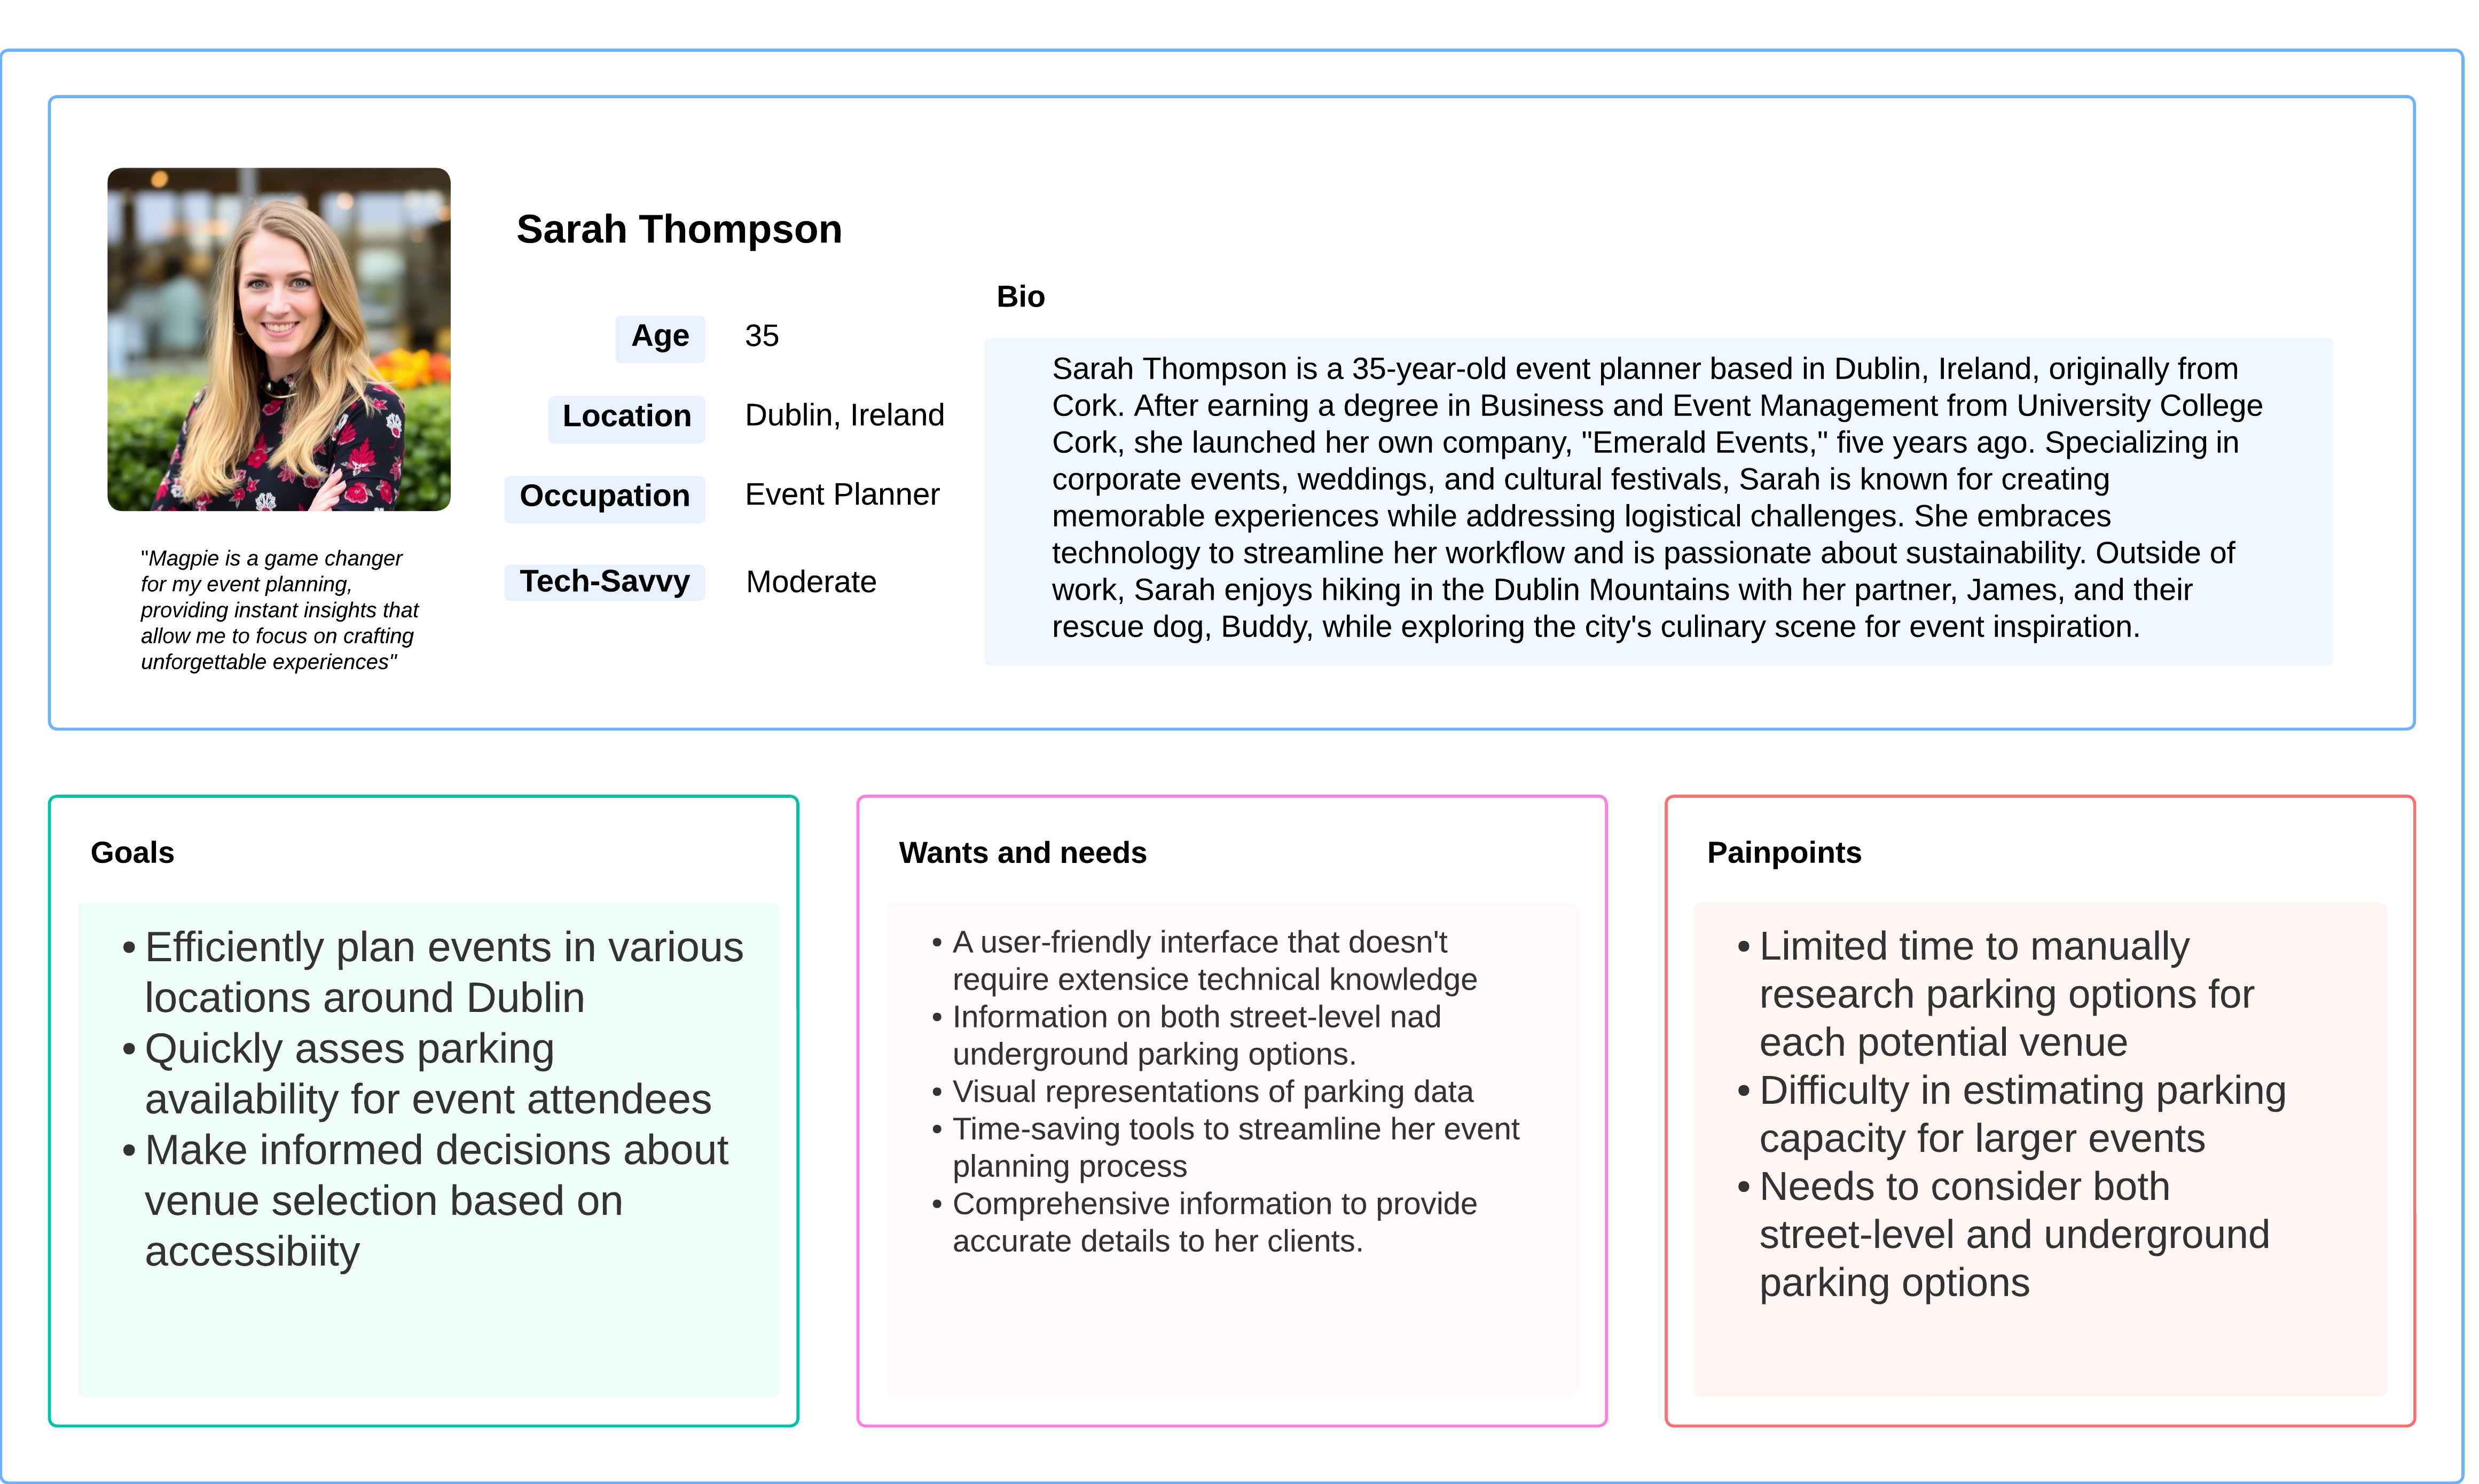
\includegraphics[width=0.8\textwidth]{images/sarah-thompson-userpersona.png}
    \caption{User persona - Sarah Thompson}
\end{figure}
Sarah thompson is a 35 year old CEO of an event's planning company based in Dublin, Ireland. She specializes in corporate events and weddings, and is known for creating memorable experiences while addressing key logistical challenges such as venue selection, catering, accessibility and transportation. She represents our secondary target user.\\
Currently, she faces many challenges planning events within Dublin city. She has limited time to manually research transport and parking options and to visually assess the accessibility of a possible venue.\\
She's looking for a tool that will give her a visual overview of transportation and parking options in an area, with additional information on their location  \& their quantity. She also needs something quick and easy to use!

\subsection{Why are they important?}
Urban Planners are crucial for the holistic development of cities and towns.
They ensure that urban development is sustainable, balancing economic growth and
environmental protection. Urban planners guide cities towards more efficient
uses of land, better transport systems, and overall increasing the quality of
life of residents.

By planning for current and future needs, Urban Planners help mitigate urban
challenges such as congestion, pollution, and lack of infrastructure. Their role
is essential for ensuring that urban areas can meet the demands of growing
populations, while maintaining standard of living and environmental
sustainability.

\subsection{What problem are we solving?}
Urban Planners often face challenges with accessing and analysing data. Data is
typically siloed, making it difficult to access and analyse. This can compromise
their capacity to make informed decisions. Our project aims to address the
difficulty in accessing and analysing data, by providing a platform that
aggregates data from multiple sources.

We aim to provide Urban Planners with a tool that allows them to access this
information in a single, easy to use, platform. This will allow Urban Planners
to streamline the initial phases of their work, decreasing the time spent on
data collection and increasing the time spent on analysis and decision making.

\subsection{Market analysis}
The identification of our target user was made possible through a exploratory work done at the beginning of the project timeline.\\
A market research survey was conducted to answer key demographic \& product questions:
\begin{enumerate}
    \item Who is our primary target user?
    \item What kind of amenity data do they access and how?
    \item What devices/tools do they primarily use?
    \item Are they satisfied with those tools?
    \item Would they consider Magpie useful in filling the gaps in their toolset?
\end{enumerate}

\newpage{}